\documentclass[12pt,a4paper]{article}
\usepackage[utf8]{inputenc}
\usepackage{graphicx}
\usepackage{amsmath}
\usepackage{amsfonts}
\usepackage{hyperref}
\usepackage{float}
\usepackage{listings}
\usepackage{xcolor}
\usepackage{verbatim}


% Listings settings for Python code
\lstset{
    language=Python,
    basicstyle=\ttfamily\small,
    keywordstyle=\color{blue}\bfseries,
    stringstyle=\color{red},
    commentstyle=\color{green!70!black},
    numberstyle=\tiny\color{gray},
    numbers=left,
    stepnumber=1,
    numbersep=8pt,
    showspaces=false,
    showstringspaces=false,
    frame=single,
    breaklines=true,
    breakatwhitespace=true,
    tabsize=4,
    captionpos=b
}

\title{Emergency Response: Cooperation and Coordination Mechanisms in Multi-Agent Systems}
\author{Your Name}
\date{\today}

\begin{document}

\maketitle
\tableofcontents
\newpage

\section{Introduction}
In this report, we present the proposed cooperation and coordination mechanisms for the CrewAI emergency response problem. The mechanisms are structured into three main components:
\begin{enumerate}
    \item Process Definition for individual crews.
    \item Pydantic Outputs for structured data handling.
    \item Agent Interaction between different crews.
\end{enumerate}



\section{Process Definition}

\subsection{Public Communication Crew Sequential Process}

The Public Communication Crew operates within a structured sequential process to ensure efficient and accurate communication of fire incident reports to the public. Each task is assigned to a specific agent with well-defined responsibilities, as detailed below:

\begin{enumerate}
	\item \textbf{Receive Report:} The \textit{Communication Operator} obtains the fire incident report in Markdown format. This serves as the starting point for the process and can filter any information that is not relevant for this crew.
	\item \textbf{Search Related Cases:} The \textit{Archive Keeper} searches for past incidents with similar locations or fire types. This task depends on the completion of the \textit{Receive Report} task.
	\item \textbf{Draft Initial Article:} The \textit{Article Writer} drafts an initial article based on the current report. This task also depends on the completion of the \textit{Receive Report} task.
	\item \textbf{Integrate Additional Information:} The \textit{Article Writer} integrates insights from related cases into the draft. This task requires the completion of both the \textit{Search Related Cases} and \textit{Draft Initial Article} tasks.
	\item \textbf{Review and Authorize Publication:} The \textit{Mayor} reviews the article and either authorizes publication or provides feedback for revisions. This task depends on the completion of the \textit{Integrate Additional Information} task.
	\item \textbf{Provide Social Media Feedback:} The \textit{Social Media Commentator} critiques the emergency response in a humorous yet constructive manner. This task depends on the approval of the article by the \textit{Mayor}.
\end{enumerate}

\begin{figure}[h!]
	\centering
	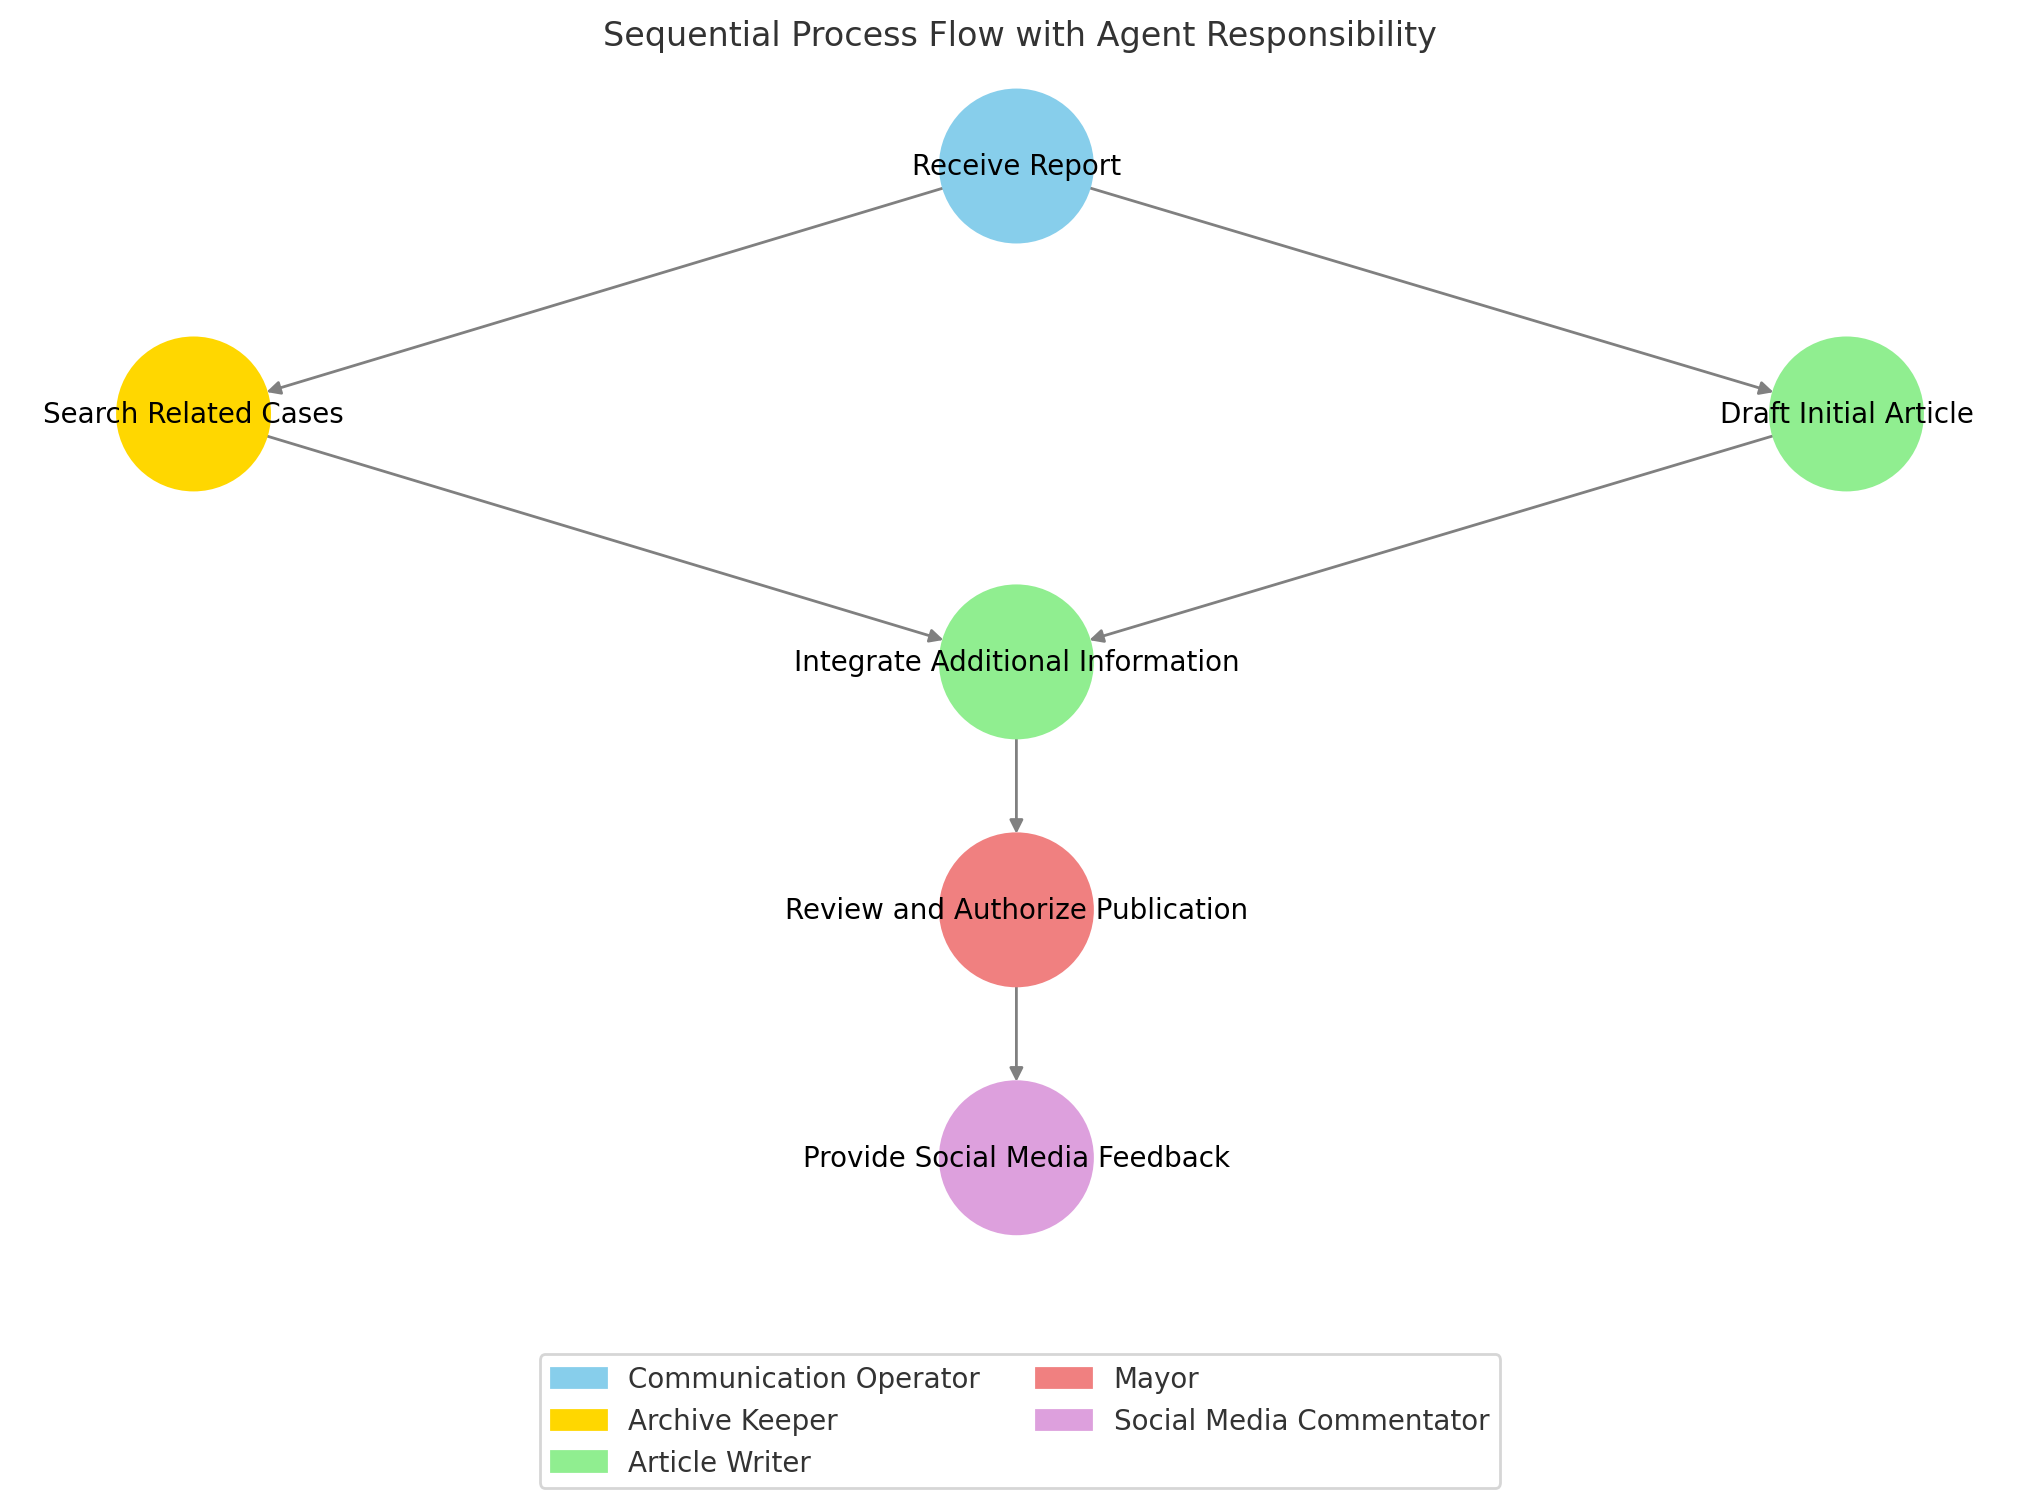
\includegraphics[width=0.9\textwidth]{figures/PC-process.png}
	\caption{Sequential Process Flow of the Public Communication Crew with Agent Responsibilities}
	\label{fig:public_comm_flow}
\end{figure}


\paragraph{Task Dependencies}
The sequential process relies on strict task dependencies to ensure an organized workflow:
\begin{itemize}
	\item \textit{Search Related Cases} and \textit{Draft Initial Article} can be executed in parallel but both depend on \textit{Receive Report}.
	\item \textit{Integrate Additional Information} requires the completion of both \textit{Search Related Cases} and \textit{Draft Initial Article}.
	\item \textit{Review and Authorize Publication} depends on \textit{Integrate Additional Information}.
	\item \textit{Provide Social Media Feedback} requires article approval from the \textit{Mayor}.
\end{itemize}

The visual representation in Figure~\ref{fig:public_comm_flow} highlights these dependencies and assigns colors to denote the responsible agents, ensuring clarity and accountability.





\section{Pydantic Outputs}
Structured outputs are essential for ensuring clarity and consistency in task execution. Below are listed the Pydantic models used in the system.

\subsection{Pydantic Outputs for Public Communication Crew}

Structured outputs are crucial for ensuring clarity, consistency, and seamless integration across tasks. Below are the Pydantic models designed for the tasks in the Public Communication Crew process:

\subsubsection{Receive Report Task Output}
\begin{lstlisting}[caption={Pydantic model for Receive Report Task Output}]
from pydantic import BaseModel

class ReceiveReportOutput(BaseModel):
    report_id: str
    location: str
    fire_type: str
    timestamp: str
    markdown_content: str
\end{lstlisting}

\subsubsection{Search Related Cases Task Output}
\begin{lstlisting}[caption={Pydantic model for Search Related Cases Task Output}]
from pydantic import BaseModel
from typing import List

class RelatedCase(BaseModel):
    case_id: str
    location: str
    fire_type: str
    summary: str

class SearchRelatedCasesOutput(BaseModel):
    related_cases: List[RelatedCase]
    total_cases: int
\end{lstlisting}

\subsubsection{Draft Initial Article Task Output}
\begin{lstlisting}[caption={Pydantic model for Draft Initial Article Task Output}]
from pydantic import BaseModel

class DraftArticleOutput(BaseModel):
    title: str
    draft: str
    author: str
\end{lstlisting}

\subsubsection{Integrate Additional Information Task Output}
\begin{lstlisting}[caption={Pydantic model for Integrate Additional Information Task Output}]
from pydantic import BaseModel

class IntegratedArticleOutput(BaseModel):
    draft: str
    integrated_sources: list[str]
\end{lstlisting}

\subsubsection{Review and Authorize Publication Task Output}
\begin{lstlisting}[caption={Pydantic model for Review and Authorize Publication Task Output}]
from pydantic import BaseModel

class ReviewOutput(BaseModel):
    approved: bool
    comments: str
    draft: str
\end{lstlisting}

\subsubsection{Provide Social Media Feedback Task Output}
\begin{lstlisting}[caption={Pydantic model for Provide Social Media Feedback Task Output}]
from pydantic import BaseModel

class SocialMediaFeedbackOutput(BaseModel):
    feedback: str
    draft: str
    approved: bool
    comments: str
\end{lstlisting}

\paragraph{Summary of Outputs}
\begin{itemize}
    \item \textbf{Receive Report Task Output:} Captures the initial fire incident report relevant details.
    \item \textbf{Search Related Cases Task Output:} Retrieves relevant historical cases for contextualization.
    \item \textbf{Draft Initial Article Task Output:} Records the initial draft content.
    \item \textbf{Integrate Additional Information Task Output:} Updates the draft with integrated sources and revisions.
    \item \textbf{Review and Authorize Publication Task Output:} Specifies the review status and comments from the Mayor.
    \item \textbf{Provide Social Media Feedback Task Output:} Details feedback posted on social media platforms, he can critize the mayor's decission.
\end{itemize}



\section{Agent Interaction}
\subsection{Interaction Flow}
Interaction between crews is designed using a flow-based approach:
\begin{itemize}
    \item The Search and Rescue Crew provides victim data to the Medical Response Crew.
    \item A **Router** determines the priority of medical cases based on data received.
\end{itemize}

\subsection{Router Implementation}
The router ensures tasks are efficiently allocated:
\begin{lstlisting}[caption={Router Implementation for Task Allocation}]
def router(victim_data):
    if victim_data["priority"] == 1:
        return "Critical Response Team"
    else:
        return "General Response Team"
\end{lstlisting}

\subsection{Communication Mechanism}
Agents communicate using a message-passing protocol to ensure scalability. An example interaction is illustrated in Figure~\ref{fig:interaction}.

\begin{comment}
\begin{figure}[H]
\centering
\includegraphics[width=0.8\textwidth]{interaction_flow.png}
\caption{Interaction Flow Between Crews}
\label{fig:interaction}
\end{figure}
\end{comment}


\section{Conclusion}
This report outlines the proposed cooperation and coordination mechanisms for the CrewAI MAS. Future work includes extending the interaction model to include additional agent types and testing the scalability of the system.


\end{document}
